% Created by tikzDevice version 0.12.6 on 2025-12-11 06:40:58
% !TEX encoding = UTF-8 Unicode
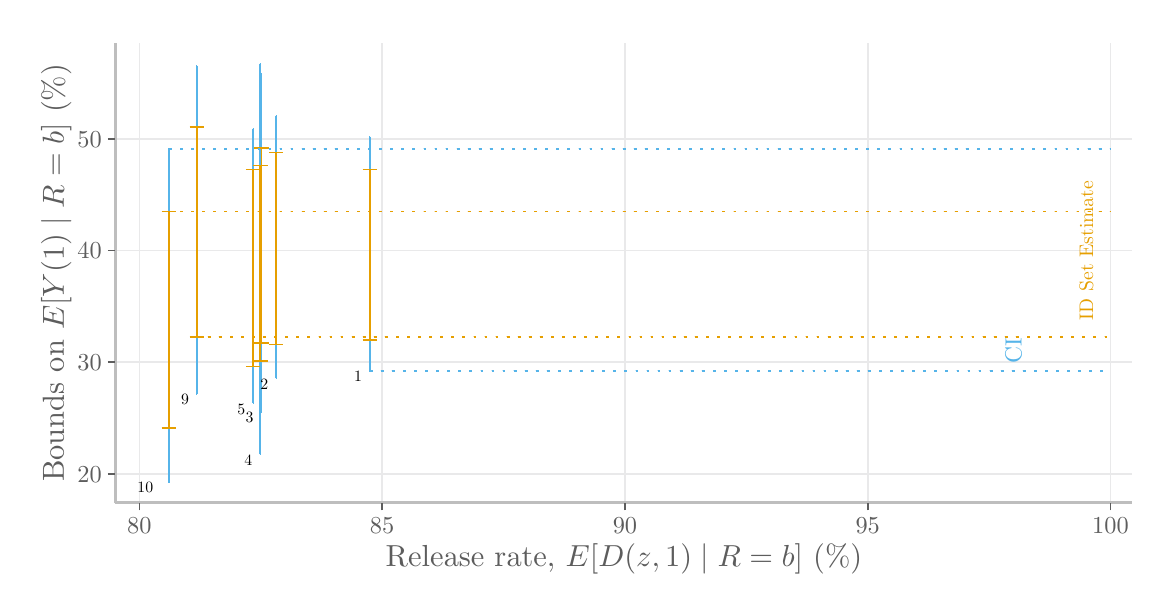
\begin{tikzpicture}[x=1pt,y=1pt]
\definecolor{fillColor}{RGB}{255,255,255}
\path[use as bounding box,fill=fillColor,fill opacity=0.00] (0,0) rectangle (404.71,202.36);
\begin{scope}
\path[clip] (  0.00,  0.00) rectangle (404.71,202.36);
\definecolor{drawColor}{RGB}{255,255,255}
\definecolor{fillColor}{RGB}{255,255,255}

\path[draw=drawColor,line width= 0.6pt,line join=round,line cap=round,fill=fillColor] (  0.00,  0.00) rectangle (404.71,202.36);
\end{scope}
\begin{scope}
\path[clip] ( 31.71, 30.69) rectangle (399.21,196.86);
\definecolor{fillColor}{RGB}{255,255,255}

\path[fill=fillColor] ( 31.71, 30.69) rectangle (399.21,196.86);
\definecolor{drawColor}{RGB}{233,233,234}

\path[draw=drawColor,line width= 0.6pt,line join=round] ( 31.71, 41.14) --
	(399.21, 41.14);

\path[draw=drawColor,line width= 0.6pt,line join=round] ( 31.71, 81.48) --
	(399.21, 81.48);

\path[draw=drawColor,line width= 0.6pt,line join=round] ( 31.71,121.81) --
	(399.21,121.81);

\path[draw=drawColor,line width= 0.6pt,line join=round] ( 31.71,162.15) --
	(399.21,162.15);

\path[draw=drawColor,line width= 0.6pt,line join=round] ( 40.36, 30.69) --
	( 40.36,196.86);

\path[draw=drawColor,line width= 0.6pt,line join=round] (128.09, 30.69) --
	(128.09,196.86);

\path[draw=drawColor,line width= 0.6pt,line join=round] (215.82, 30.69) --
	(215.82,196.86);

\path[draw=drawColor,line width= 0.6pt,line join=round] (303.55, 30.69) --
	(303.55,196.86);

\path[draw=drawColor,line width= 0.6pt,line join=round] (391.28, 30.69) --
	(391.28,196.86);
\definecolor{drawColor}{RGB}{86,180,233}

\path[draw=drawColor,line width= 0.6pt,line join=round] ( 60.91,188.59) --
	( 61.32,188.59);

\path[draw=drawColor,line width= 0.6pt,line join=round] ( 61.11,188.59) --
	( 61.11, 69.97);

\path[draw=drawColor,line width= 0.6pt,line join=round] ( 60.91, 69.97) --
	( 61.32, 69.97);

\path[draw=drawColor,line width= 0.6pt,line join=round] ( 50.85,158.44) --
	( 51.25,158.44);

\path[draw=drawColor,line width= 0.6pt,line join=round] ( 51.05,158.44) --
	( 51.05, 38.24);

\path[draw=drawColor,line width= 0.6pt,line join=round] ( 50.85, 38.24) --
	( 51.25, 38.24);

\path[draw=drawColor,line width= 0.6pt,line join=round] (123.44,163.01) --
	(123.84,163.01);

\path[draw=drawColor,line width= 0.6pt,line join=round] (123.64,163.01) --
	(123.64, 78.38);

\path[draw=drawColor,line width= 0.6pt,line join=round] (123.44, 78.38) --
	(123.84, 78.38);

\path[draw=drawColor,line width= 0.6pt,line join=round] ( 84.28,185.50) --
	( 84.69,185.50);

\path[draw=drawColor,line width= 0.6pt,line join=round] ( 84.49,185.50) --
	( 84.49, 63.52);

\path[draw=drawColor,line width= 0.6pt,line join=round] ( 84.28, 63.52) --
	( 84.69, 63.52);

\path[draw=drawColor,line width= 0.6pt,line join=round] ( 83.83,189.30) --
	( 84.24,189.30);

\path[draw=drawColor,line width= 0.6pt,line join=round] ( 84.04,189.30) --
	( 84.04, 48.16);

\path[draw=drawColor,line width= 0.6pt,line join=round] ( 83.83, 48.16) --
	( 84.24, 48.16);

\path[draw=drawColor,line width= 0.6pt,line join=round] ( 81.27,165.68) --
	( 81.67,165.68);

\path[draw=drawColor,line width= 0.6pt,line join=round] ( 81.47,165.68) --
	( 81.47, 66.63);

\path[draw=drawColor,line width= 0.6pt,line join=round] ( 81.27, 66.63) --
	( 81.67, 66.63);

\path[draw=drawColor,line width= 0.6pt,line join=round] ( 89.56,170.43) --
	( 89.97,170.43);

\path[draw=drawColor,line width= 0.6pt,line join=round] ( 89.76,170.43) --
	( 89.76, 75.64);

\path[draw=drawColor,line width= 0.6pt,line join=round] ( 89.56, 75.64) --
	( 89.97, 75.64);
\definecolor{drawColor}{RGB}{230,159,0}

\path[draw=drawColor,line width= 0.6pt,line join=round] ( 58.48,166.52) --
	( 63.75,166.52);

\path[draw=drawColor,line width= 0.6pt,line join=round] ( 61.11,166.52) --
	( 61.11, 90.61);

\path[draw=drawColor,line width= 0.6pt,line join=round] ( 58.48, 90.61) --
	( 63.75, 90.61);

\path[draw=drawColor,line width= 0.6pt,line join=round] ( 48.42,135.90) --
	( 53.68,135.90);

\path[draw=drawColor,line width= 0.6pt,line join=round] ( 51.05,135.90) --
	( 51.05, 57.68);

\path[draw=drawColor,line width= 0.6pt,line join=round] ( 48.42, 57.68) --
	( 53.68, 57.68);

\path[draw=drawColor,line width= 0.6pt,line join=round] (121.01,151.07) --
	(126.27,151.07);

\path[draw=drawColor,line width= 0.6pt,line join=round] (123.64,151.07) --
	(123.64, 89.54);

\path[draw=drawColor,line width= 0.6pt,line join=round] (121.01, 89.54) --
	(126.27, 89.54);

\path[draw=drawColor,line width= 0.6pt,line join=round] ( 81.86,158.85) --
	( 87.12,158.85);

\path[draw=drawColor,line width= 0.6pt,line join=round] ( 84.49,158.85) --
	( 84.49, 88.32);

\path[draw=drawColor,line width= 0.6pt,line join=round] ( 81.86, 88.32) --
	( 87.12, 88.32);

\path[draw=drawColor,line width= 0.6pt,line join=round] ( 81.40,152.55) --
	( 86.67,152.55);

\path[draw=drawColor,line width= 0.6pt,line join=round] ( 84.04,152.55) --
	( 84.04, 81.92);

\path[draw=drawColor,line width= 0.6pt,line join=round] ( 81.40, 81.92) --
	( 86.67, 81.92);

\path[draw=drawColor,line width= 0.6pt,line join=round] ( 78.84,151.14) --
	( 84.10,151.14);

\path[draw=drawColor,line width= 0.6pt,line join=round] ( 81.47,151.14) --
	( 81.47, 79.92);

\path[draw=drawColor,line width= 0.6pt,line join=round] ( 78.84, 79.92) --
	( 84.10, 79.92);

\path[draw=drawColor,line width= 0.6pt,line join=round] ( 87.13,157.23) --
	( 92.40,157.23);

\path[draw=drawColor,line width= 0.6pt,line join=round] ( 89.76,157.23) --
	( 89.76, 87.92);

\path[draw=drawColor,line width= 0.6pt,line join=round] ( 87.13, 87.92) --
	( 92.40, 87.92);
\definecolor{drawColor}{RGB}{0,0,0}

\node[text=drawColor,anchor=base east,inner sep=0pt, outer sep=0pt, scale=  0.57] at ( 58.27, 66.05) {9};

\node[text=drawColor,anchor=base east,inner sep=0pt, outer sep=0pt, scale=  0.57] at ( 45.36, 34.32) {10};

\node[text=drawColor,anchor=base east,inner sep=0pt, outer sep=0pt, scale=  0.57] at (120.79, 74.46) {1};

\node[text=drawColor,anchor=base east,inner sep=0pt, outer sep=0pt, scale=  0.57] at ( 81.64, 59.60) {3};

\node[text=drawColor,anchor=base east,inner sep=0pt, outer sep=0pt, scale=  0.57] at ( 81.19, 44.24) {4};

\node[text=drawColor,anchor=base east,inner sep=0pt, outer sep=0pt, scale=  0.57] at ( 78.63, 62.71) {5};

\node[text=drawColor,anchor=base east,inner sep=0pt, outer sep=0pt, scale=  0.57] at ( 86.92, 71.72) {2};
\definecolor{drawColor}{RGB}{230,159,0}

\path[draw=drawColor,line width= 0.6pt,dash pattern=on 1pt off 3pt ,line join=round] ( 61.11, 90.61) -- (391.28, 90.61);

\path[draw=drawColor,line width= 0.6pt,dash pattern=on 1pt off 3pt ,line join=round] ( 61.11, 90.61) -- (391.28, 90.61);

\path[draw=drawColor,line width= 0.6pt,dash pattern=on 1pt off 3pt ,line join=round] ( 61.11, 90.61) -- (391.28, 90.61);

\path[draw=drawColor,line width= 0.6pt,dash pattern=on 1pt off 3pt ,line join=round] ( 61.11, 90.61) -- (391.28, 90.61);

\path[draw=drawColor,line width= 0.6pt,dash pattern=on 1pt off 3pt ,line join=round] ( 61.11, 90.61) -- (391.28, 90.61);

\path[draw=drawColor,line width= 0.6pt,dash pattern=on 1pt off 3pt ,line join=round] ( 61.11, 90.61) -- (391.28, 90.61);

\path[draw=drawColor,line width= 0.6pt,dash pattern=on 1pt off 3pt ,line join=round] ( 61.11, 90.61) -- (391.28, 90.61);

\path[draw=drawColor,line width= 0.6pt,dash pattern=on 1pt off 3pt ,line join=round] ( 51.05,135.90) -- (391.28,135.90);

\path[draw=drawColor,line width= 0.6pt,dash pattern=on 1pt off 3pt ,line join=round] ( 51.05,135.90) -- (391.28,135.90);

\path[draw=drawColor,line width= 0.6pt,dash pattern=on 1pt off 3pt ,line join=round] ( 51.05,135.90) -- (391.28,135.90);

\path[draw=drawColor,line width= 0.6pt,dash pattern=on 1pt off 3pt ,line join=round] ( 51.05,135.90) -- (391.28,135.90);

\path[draw=drawColor,line width= 0.6pt,dash pattern=on 1pt off 3pt ,line join=round] ( 51.05,135.90) -- (391.28,135.90);

\path[draw=drawColor,line width= 0.6pt,dash pattern=on 1pt off 3pt ,line join=round] ( 51.05,135.90) -- (391.28,135.90);

\path[draw=drawColor,line width= 0.6pt,dash pattern=on 1pt off 3pt ,line join=round] ( 51.05,135.90) -- (391.28,135.90);
\definecolor{drawColor}{RGB}{86,180,233}

\path[draw=drawColor,line width= 0.6pt,dash pattern=on 1pt off 3pt ,line join=round] (123.64, 78.38) -- (391.28, 78.38);

\path[draw=drawColor,line width= 0.6pt,dash pattern=on 1pt off 3pt ,line join=round] (123.64, 78.38) -- (391.28, 78.38);

\path[draw=drawColor,line width= 0.6pt,dash pattern=on 1pt off 3pt ,line join=round] (123.64, 78.38) -- (391.28, 78.38);

\path[draw=drawColor,line width= 0.6pt,dash pattern=on 1pt off 3pt ,line join=round] (123.64, 78.38) -- (391.28, 78.38);

\path[draw=drawColor,line width= 0.6pt,dash pattern=on 1pt off 3pt ,line join=round] (123.64, 78.38) -- (391.28, 78.38);

\path[draw=drawColor,line width= 0.6pt,dash pattern=on 1pt off 3pt ,line join=round] (123.64, 78.38) -- (391.28, 78.38);

\path[draw=drawColor,line width= 0.6pt,dash pattern=on 1pt off 3pt ,line join=round] (123.64, 78.38) -- (391.28, 78.38);

\path[draw=drawColor,line width= 0.6pt,dash pattern=on 1pt off 3pt ,line join=round] ( 51.05,158.44) -- (391.28,158.44);

\path[draw=drawColor,line width= 0.6pt,dash pattern=on 1pt off 3pt ,line join=round] ( 51.05,158.44) -- (391.28,158.44);

\path[draw=drawColor,line width= 0.6pt,dash pattern=on 1pt off 3pt ,line join=round] ( 51.05,158.44) -- (391.28,158.44);

\path[draw=drawColor,line width= 0.6pt,dash pattern=on 1pt off 3pt ,line join=round] ( 51.05,158.44) -- (391.28,158.44);

\path[draw=drawColor,line width= 0.6pt,dash pattern=on 1pt off 3pt ,line join=round] ( 51.05,158.44) -- (391.28,158.44);

\path[draw=drawColor,line width= 0.6pt,dash pattern=on 1pt off 3pt ,line join=round] ( 51.05,158.44) -- (391.28,158.44);

\path[draw=drawColor,line width= 0.6pt,dash pattern=on 1pt off 3pt ,line join=round] ( 51.05,158.44) -- (391.28,158.44);
\definecolor{drawColor}{RGB}{230,159,0}

\node[text=drawColor,rotate= 90.00,anchor=base,inner sep=0pt, outer sep=0pt, scale=  0.71] at (384.96,121.81) {ID Set Estimate};
\definecolor{drawColor}{RGB}{86,180,233}

\node[text=drawColor,rotate= 90.00,anchor=base,inner sep=0pt, outer sep=0pt, scale=  0.85] at (359.13, 85.51) {CI};
\end{scope}
\begin{scope}
\path[clip] (  0.00,  0.00) rectangle (404.71,202.36);
\definecolor{drawColor}{RGB}{190,190,190}

\path[draw=drawColor,line width= 1.1pt,line join=round] ( 31.71, 30.69) --
	( 31.71,196.86);
\end{scope}
\begin{scope}
\path[clip] (  0.00,  0.00) rectangle (404.71,202.36);
\definecolor{drawColor}{RGB}{93,93,93}

\node[text=drawColor,anchor=base east,inner sep=0pt, outer sep=0pt, scale=  0.88] at ( 26.76, 38.11) {20};

\node[text=drawColor,anchor=base east,inner sep=0pt, outer sep=0pt, scale=  0.88] at ( 26.76, 78.45) {30};

\node[text=drawColor,anchor=base east,inner sep=0pt, outer sep=0pt, scale=  0.88] at ( 26.76,118.78) {40};

\node[text=drawColor,anchor=base east,inner sep=0pt, outer sep=0pt, scale=  0.88] at ( 26.76,159.12) {50};
\end{scope}
\begin{scope}
\path[clip] (  0.00,  0.00) rectangle (404.71,202.36);
\definecolor{drawColor}{RGB}{93,93,93}

\path[draw=drawColor,line width= 0.6pt,line join=round] ( 28.96, 41.14) --
	( 31.71, 41.14);

\path[draw=drawColor,line width= 0.6pt,line join=round] ( 28.96, 81.48) --
	( 31.71, 81.48);

\path[draw=drawColor,line width= 0.6pt,line join=round] ( 28.96,121.81) --
	( 31.71,121.81);

\path[draw=drawColor,line width= 0.6pt,line join=round] ( 28.96,162.15) --
	( 31.71,162.15);
\end{scope}
\begin{scope}
\path[clip] (  0.00,  0.00) rectangle (404.71,202.36);
\definecolor{drawColor}{RGB}{190,190,190}

\path[draw=drawColor,line width= 1.1pt,line join=round] ( 31.71, 30.69) --
	(399.21, 30.69);
\end{scope}
\begin{scope}
\path[clip] (  0.00,  0.00) rectangle (404.71,202.36);
\definecolor{drawColor}{RGB}{93,93,93}

\path[draw=drawColor,line width= 0.6pt,line join=round] ( 40.36, 27.94) --
	( 40.36, 30.69);

\path[draw=drawColor,line width= 0.6pt,line join=round] (128.09, 27.94) --
	(128.09, 30.69);

\path[draw=drawColor,line width= 0.6pt,line join=round] (215.82, 27.94) --
	(215.82, 30.69);

\path[draw=drawColor,line width= 0.6pt,line join=round] (303.55, 27.94) --
	(303.55, 30.69);

\path[draw=drawColor,line width= 0.6pt,line join=round] (391.28, 27.94) --
	(391.28, 30.69);
\end{scope}
\begin{scope}
\path[clip] (  0.00,  0.00) rectangle (404.71,202.36);
\definecolor{drawColor}{RGB}{93,93,93}

\node[text=drawColor,anchor=base,inner sep=0pt, outer sep=0pt, scale=  0.88] at ( 40.36, 19.68) {80};

\node[text=drawColor,anchor=base,inner sep=0pt, outer sep=0pt, scale=  0.88] at (128.09, 19.68) {85};

\node[text=drawColor,anchor=base,inner sep=0pt, outer sep=0pt, scale=  0.88] at (215.82, 19.68) {90};

\node[text=drawColor,anchor=base,inner sep=0pt, outer sep=0pt, scale=  0.88] at (303.55, 19.68) {95};

\node[text=drawColor,anchor=base,inner sep=0pt, outer sep=0pt, scale=  0.88] at (391.28, 19.68) {100};
\end{scope}
\begin{scope}
\path[clip] (  0.00,  0.00) rectangle (404.71,202.36);
\definecolor{drawColor}{RGB}{93,93,93}

\node[text=drawColor,anchor=base,inner sep=0pt, outer sep=0pt, scale=  1.10] at (215.46,  7.64) {Release rate, $E[D(z, 1)\mid R=b]$ (\%)};
\end{scope}
\begin{scope}
\path[clip] (  0.00,  0.00) rectangle (404.71,202.36);
\definecolor{drawColor}{RGB}{93,93,93}

\node[text=drawColor,rotate= 90.00,anchor=base,inner sep=0pt, outer sep=0pt, scale=  1.10] at ( 13.08,113.77) {Bounds on $E[Y(1)\mid R=b]$  (\%)};
\end{scope}
\end{tikzpicture}
